\documentclass[../main.tex]{subfiles}
\graphicspath{{\subfix{../imgs/}}}
\begin{document}
\newpage

\chapter{The Performance Environment: A prototype}

\section{For the non-technical perfomer}
Before working on the training of the model itself, I created a prototype for the model environment and tested it against a pre-built model, \textit{Improv RNN}, from Google's Magenta Library. \textit{Improv RNN} takes in a quantized note sequence as well as an optionally provided chord progression and returns a candidate continuation of the sequence.

Within Max, I have created a patch that serves as the interface between the performer and the entire system. Max conveniently features a ``presentation mode'', that hides the intricate details of the max patch, making it particularly approachable for a non-technical performer who might use the system in the future. 

\begin{figure}[htpb]
    \centering
    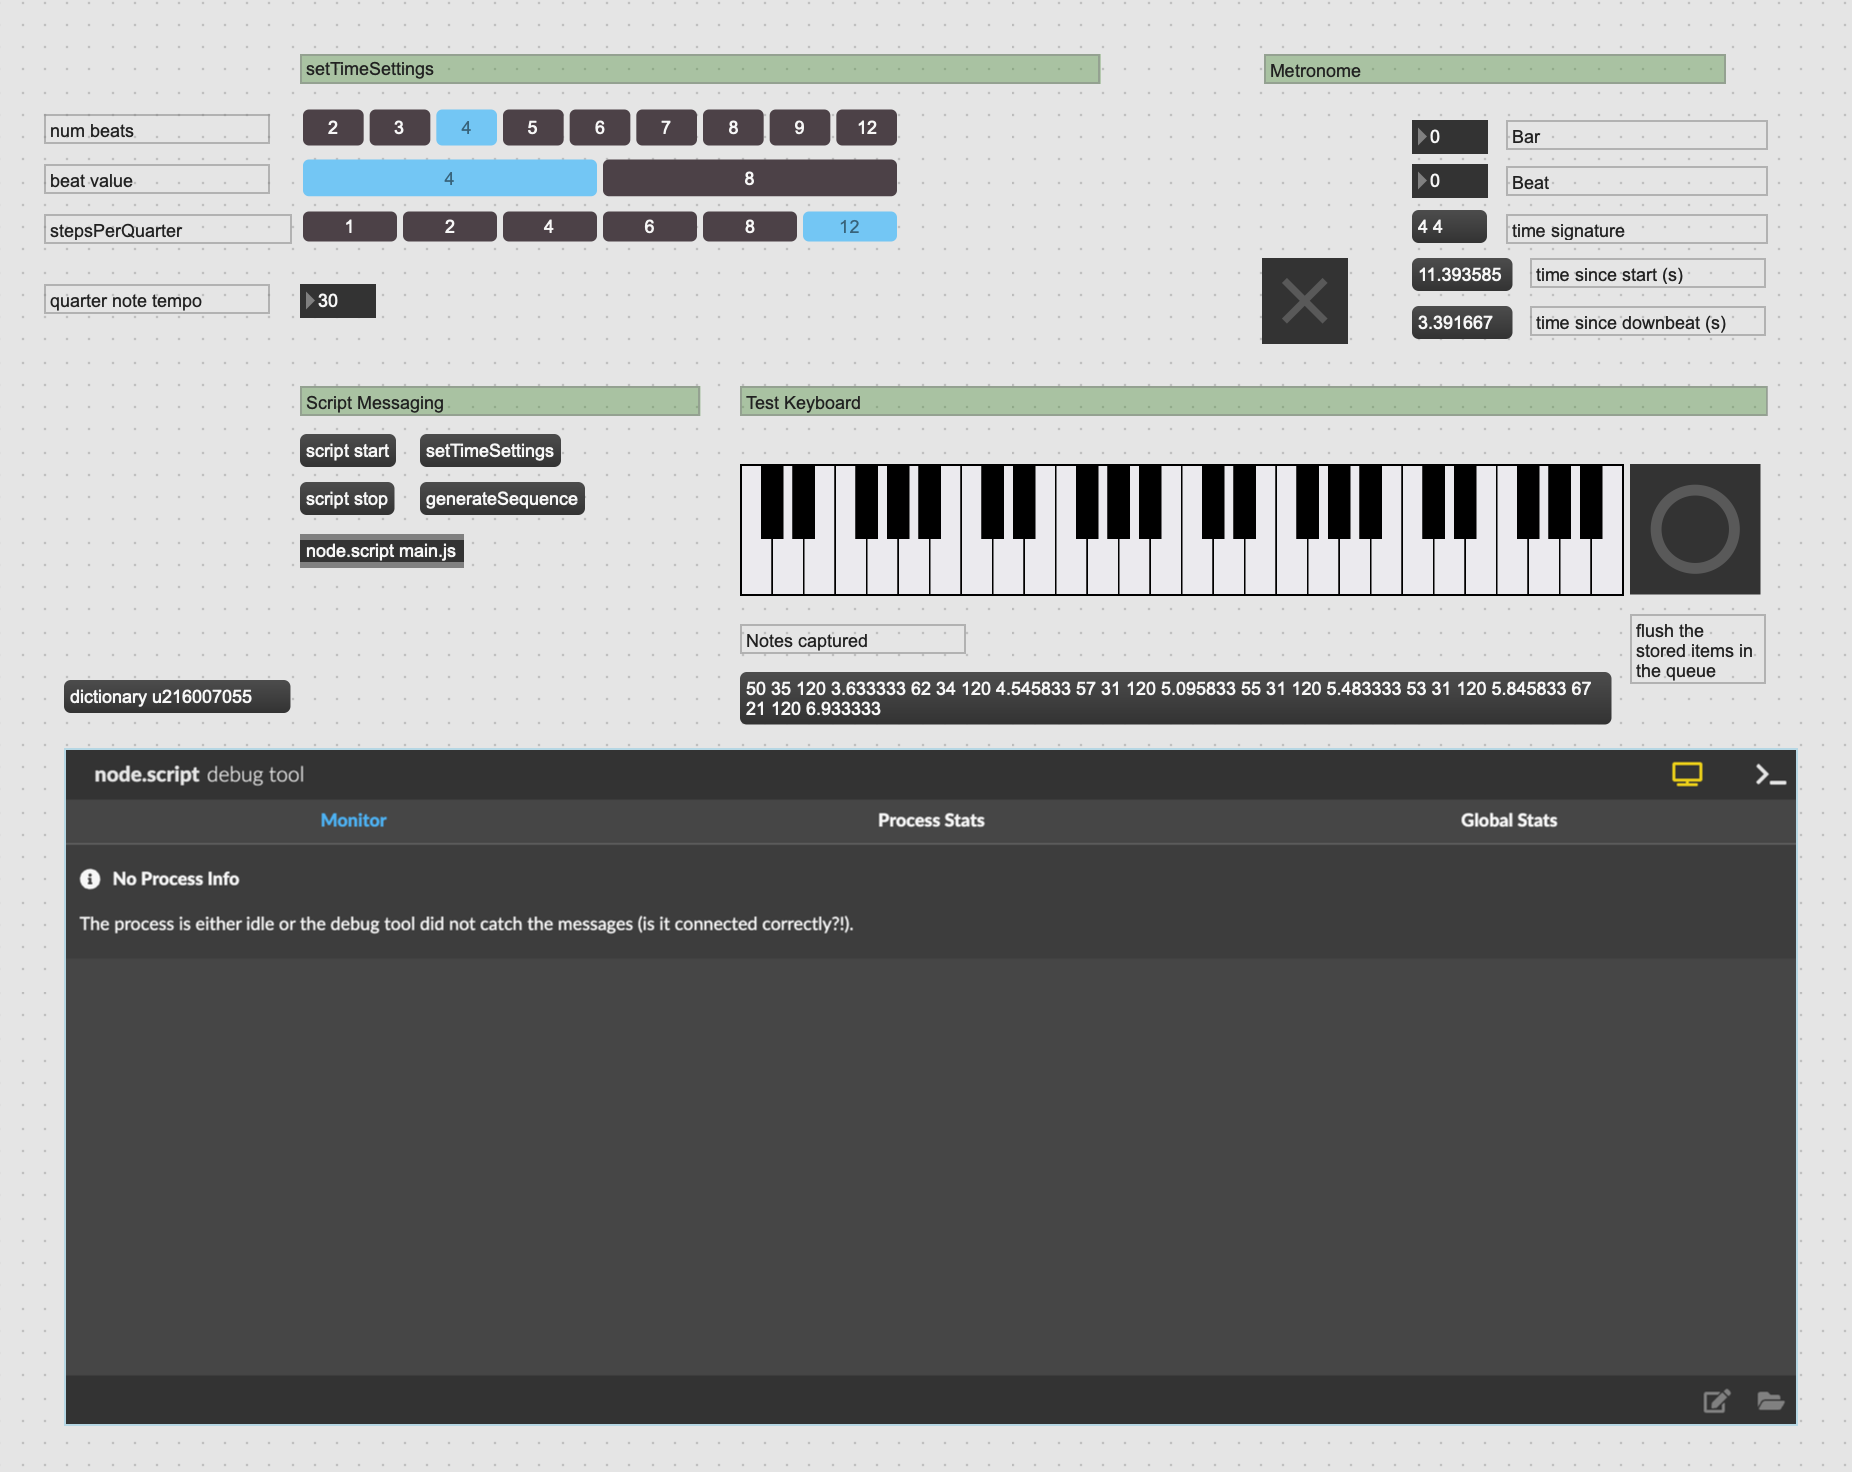
\includegraphics[width=1\textwidth]{imgs/performer_interface.png}
    \caption{Performer interface using Presentation mode in Max, which lets us selectively show Max objects whilst hiding all of the necessary ``cabling" }
    \label{fig:performer_interface}
\end{figure}

The patch has 4 distinct control sections:

\begin{enumerate}
    \item \textbf{setTimeSettings} — Here the performer can pre-set settings based on the kind of music they would like to play. This includes setting a time signature using \textit{numbeats} and  \textit{beatvalue} (eg. 9/8 would be 9 beats, each with an 8th note value). Here the performer can also alter the quarter note tempo and as well as stepsPerQuarter variable, which are required by ImprovRNN specifically to quantize an incoming note sequence. 

     \item \textbf{Script Messaging} — After the time settings have been set, the performer can start the script ``main.js", the entry point file for our Javascript interface. Can also manually call \textit{setTimeSettings} to reset the established settings if they change it once the script has already started

    \item \textbf{Metronome} — Once the script has started, the model has loaded and the time settings have been set, The performer can click the toggle within this section to start the metronome for the piece. The metronome here is created using Max's \textit{global transport} object, which is a crucial component for tracking the input midi notes.

    \item \textbf{Test Keyboard} — In its current state, the environment works with the test keyboard rendered within Max itself which is able to send out note onsets as well as note velocities. This can be readily swapped out with a pitch-tracking module. Next to the keyboard is also a ``bang" object that will manually flush our note queue for testing purposes. In reality, the note queue will automatically flush its contents to the Javascript runtime at set intervals based on the time settings set by the performer.
\end{enumerate}

\section{Technical Details of the Patch}
To send all the required information to our Javascript Runtime, I first instantiated a metronome that ticks alongside the host computer's internal clock. After the metronome has started, the \textit{global transport} object mentioned earlier is simultaneously able to keep track of the current bar and beat (based on the time settings provided) as well as the total ticks elapsed since the metronome started. 

Given that we are working with MIDI in real-time, we have to manually calculate the time data that is naturally present in a MIDI file. Every time a note is triggered via the test keyboard, we can immediately retrieve a note value as well as a velocity value. It also then uses the values from the global transport object to determine how long the note was played for, as well as the delta time between the start of the note, and the start of the bar. These four variables are packed into a queue every time a note is sounded. Every time a new bar starts, Max then flushes the note queue entirely into our Javascript Runtime. 

Our Javascript process then parses these notes into a stream of MIDI note objects, which are then quantized and passed to the model using methods from the \textit{Magenta.js} library. Note that these note objects are currently formatted to work with ImprovRNN, and the encoding proposed by Oore et al. has not yet been implemented within this environment

\begin{figure}[htpb]
    \centering
    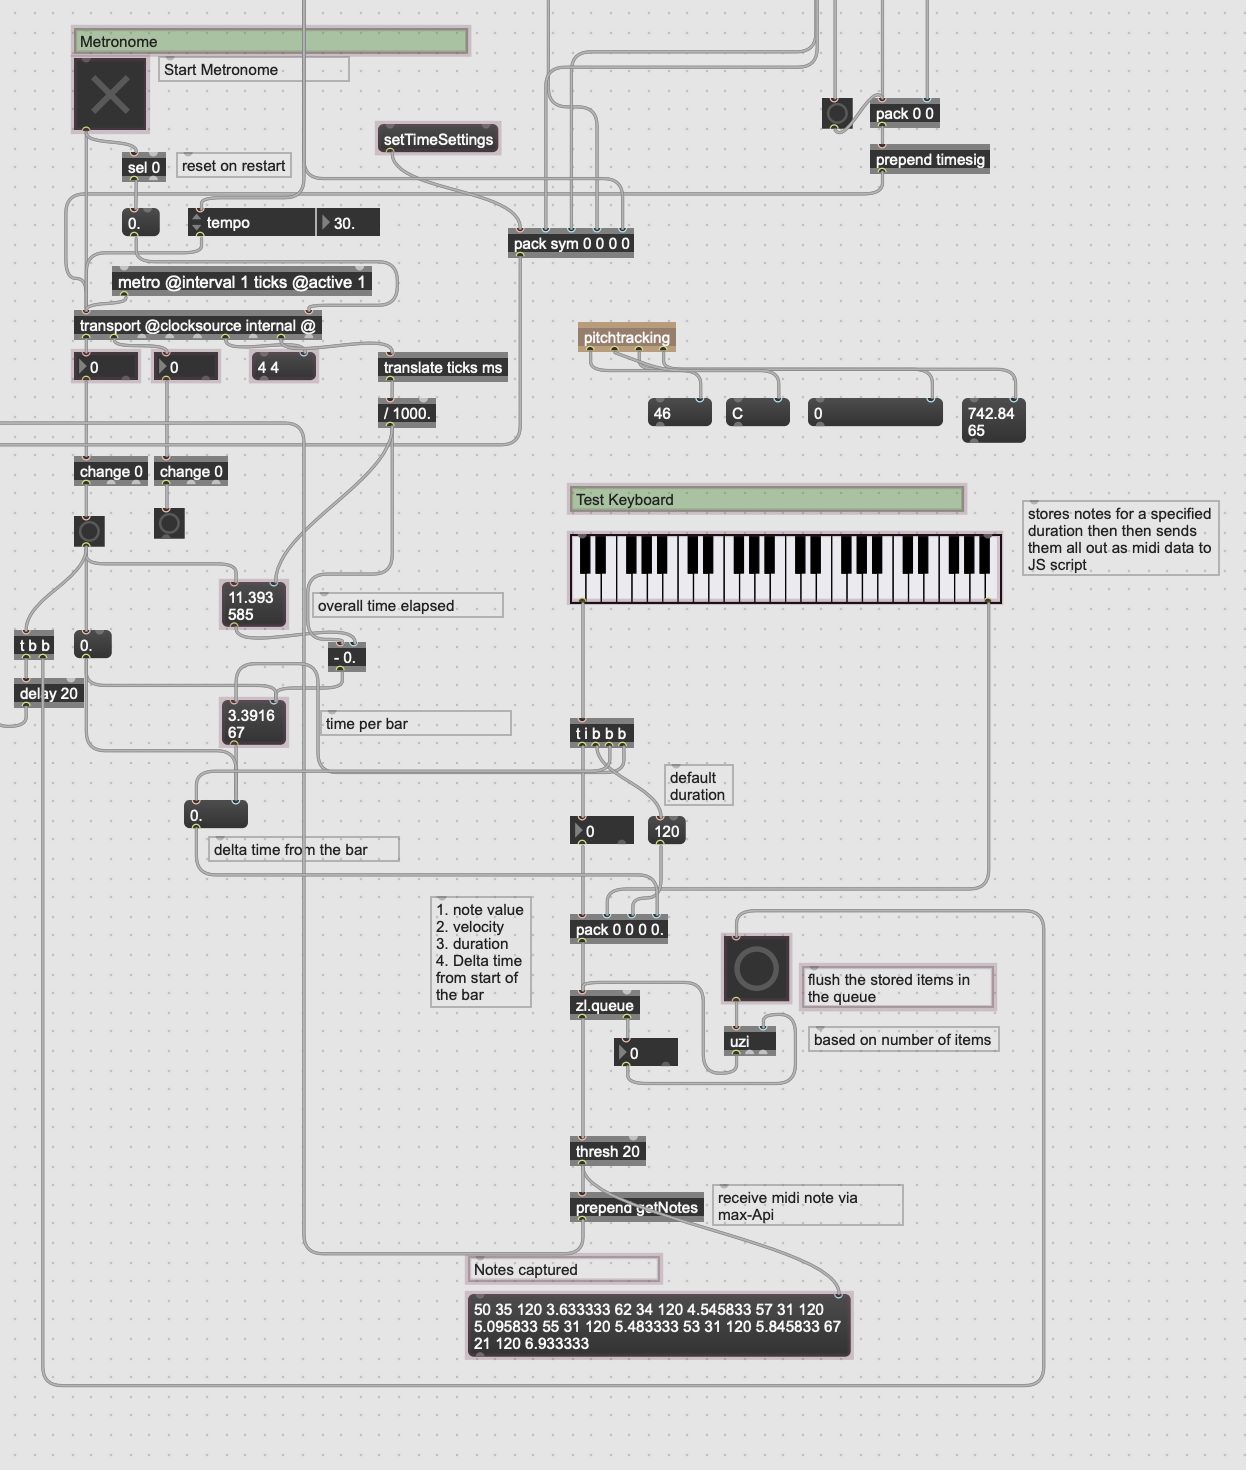
\includegraphics[width=0.9\textwidth]{imgs/note_queuing_mechanism.png}
    \caption{The Max patch collecting note events into a queue}
    \label{fig:note_queuing_mechanism}
\end{figure}

\section{Pitch Tracking}
As it currently stands, the pitch-tracking module has already been included in the patch but has not yet been connected to the patch to replace the test keyboard. The pitch-tracking module is currently built to track monophonic pitch with the \textit{Sigmund} object created by Max Miller Puckette. 

\begin{figure}[htpb]
    \centering
    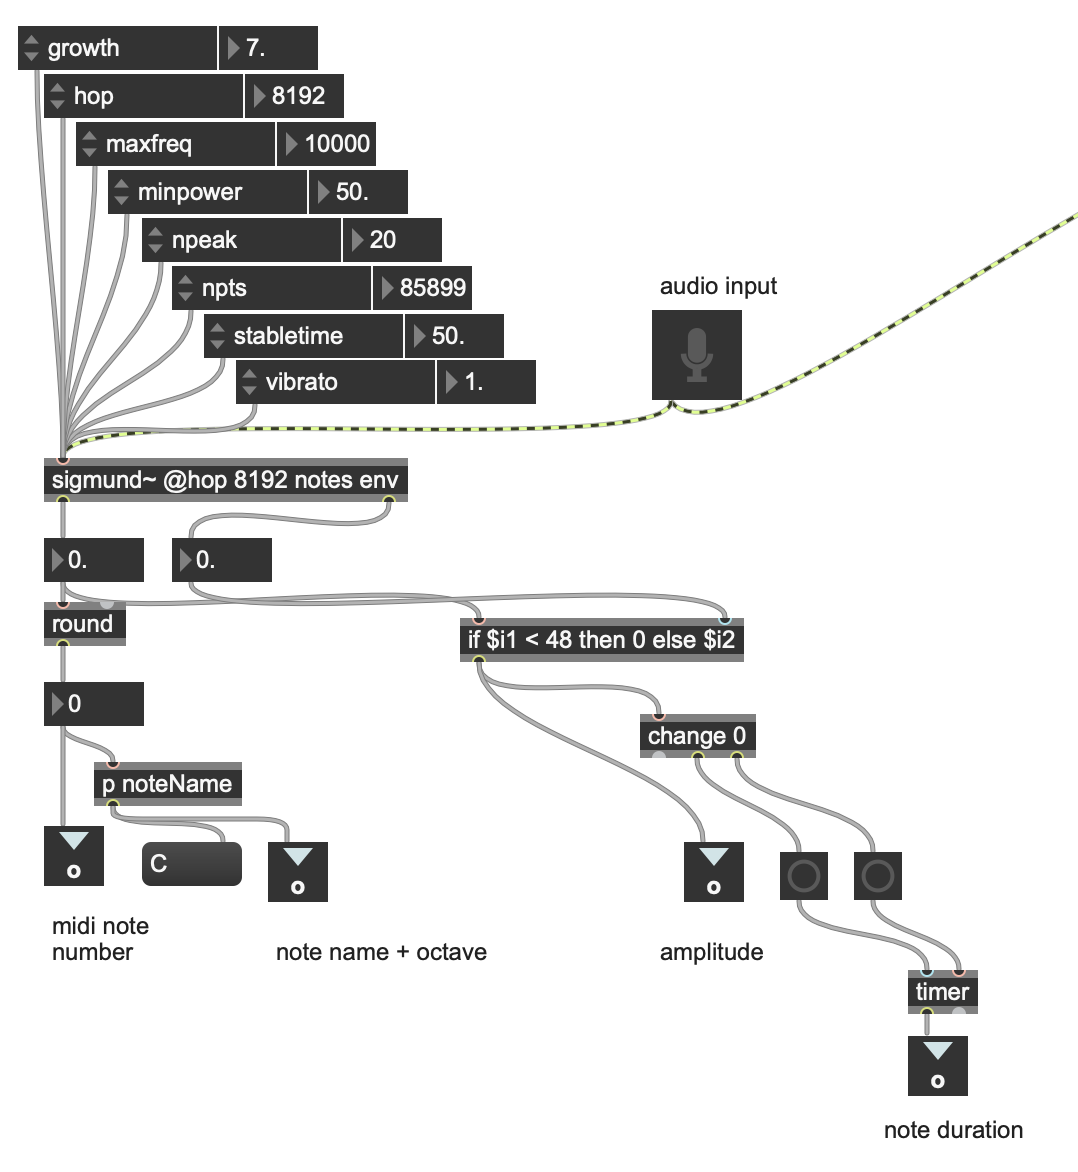
\includegraphics[width=0.8\textwidth]{imgs/pitchtracking_module.png}
    \caption{Simple Pitch-tracking with Sigmund}
    \label{fig:pitch_tracking}
\end{figure}

Given that the main goal of the project is in the Transformer model domain, it suffices to use Monophonic Pitch-tracking to evaluate our model. However, for more robust, polyphonic pitch-tracking, we may implement the method described in Robertson et al. \cite{Robertson:1} which uses harmonic partial subtraction alongside the \textit{Fiddle} object in Max.

\end{document}